%%%%%%%%%%%%%%%%%%%%%%%%%%%%%%%%%%%%%%%%%%%%%%%%%%%%%%%%%%%%%%%%%%%%%%%%%%%%%%%%%%%%%%%%%%%%%%%%%%%%%%%%%%%%%%%%%%%%%%%%%%%%%%%%%%%%%%%%%%%%%%%%%%%%%%%%%%%%%%%%%%%%%%%%%%%%%%%%%%%%%%%%%%%%
% Written By Michael Brodskiy
% Class: AP Environmental Science
% Instructor: Mrs. Stansbury
%%%%%%%%%%%%%%%%%%%%%%%%%%%%%%%%%%%%%%%%%%%%%%%%%%%%%%%%%%%%%%%%%%%%%%%%%%%%%%%%%%%%%%%%%%%%%%%%%%%%%%%%%%%%%%%%%%%%%%%%%%%%%%%%%%%%%%%%%%%%%%%%%%%%%%%%%%%%%%%%%%%%%%%%%%%%%%%%%%%%%%%%%%%%

\documentclass[12pt]{article} 
\usepackage{alphalph}
\usepackage[utf8]{inputenc}
\usepackage[russian,english]{babel}
\usepackage{titling}
\usepackage{amsmath}
\usepackage{graphicx}
\usepackage{enumitem}
\usepackage{amssymb}
\usepackage{physics}
\usepackage{tikz}
\usepackage{mathdots}
\usepackage{yhmath}
\usepackage{cancel}
\usepackage{color}
\usepackage{siunitx}
\usepackage{array}
\usepackage{multirow}
\usepackage{gensymb}
\usepackage{tabularx}
\usepackage{booktabs}
\usepackage{soul}
\usepackage{color, colortbl}
\usetikzlibrary{fadings}
\usetikzlibrary{patterns}
\usetikzlibrary{shadows.blur}
\usetikzlibrary{shapes}
\usepackage[super]{nth}
\usepackage{expl3}
\usepackage[version=4]{mhchem}
\usepackage{hpstatement}
\usepackage{rsphrase}
\usepackage{everysel}
\usepackage{ragged2e}
\usepackage{geometry}
\usepackage{fancyhdr}
\usepackage{cancel}
\geometry{top=1.0in,bottom=1.0in,left=1.0in,right=1.0in}
\newcommand{\subtitle}[1]{%
  \posttitle{%
    \par\end{center}
    \begin{center}\large#1\end{center}
    \vskip0.5em}%

}
\usepackage{hyperref}
\hypersetup{
colorlinks=true,
linkcolor=blue,
filecolor=magenta,      
urlcolor=blue,
citecolor=blue,
}

\urlstyle{same}

\definecolor{BurntOrange}{rgb}{0.85, 0.6, 0.3}
\definecolor{Gray}{gray}{.5}

\title{APES Final Project:}
\subtitle{Crystal Ball Math: Predicting Population Growth with Models}
\date{Period 1}
\author{Autumn Hamlin \& Michael Brodskiy\\ \small Instructor: Mrs. Stansbury}

\begin{document}

\maketitle

\newpage

\tableofcontents

\newpage

\section{Research Data}

\begin{center}
  \begin{tabular}{| c | c | c |}
    \hline
    \rowcolor{BurntOrange} Animal & Carrying Capacity & Growth Rate\\
    \hline
    \rowcolor{Gray!35} Gray Wolf & 400 & 21\%\\
    \hline
    Moose & 840 & 25\%\\
    \hline
    \rowcolor{Gray!35} Woodland Caribou & 200 & 24.5\%\\
    \hline
    Elephant & 7,500 & 15\%\\
    \hline
  \end{tabular}
\end{center}

\section{Case Studies}

\subsection{Gray Wolf}

\begin{center}
  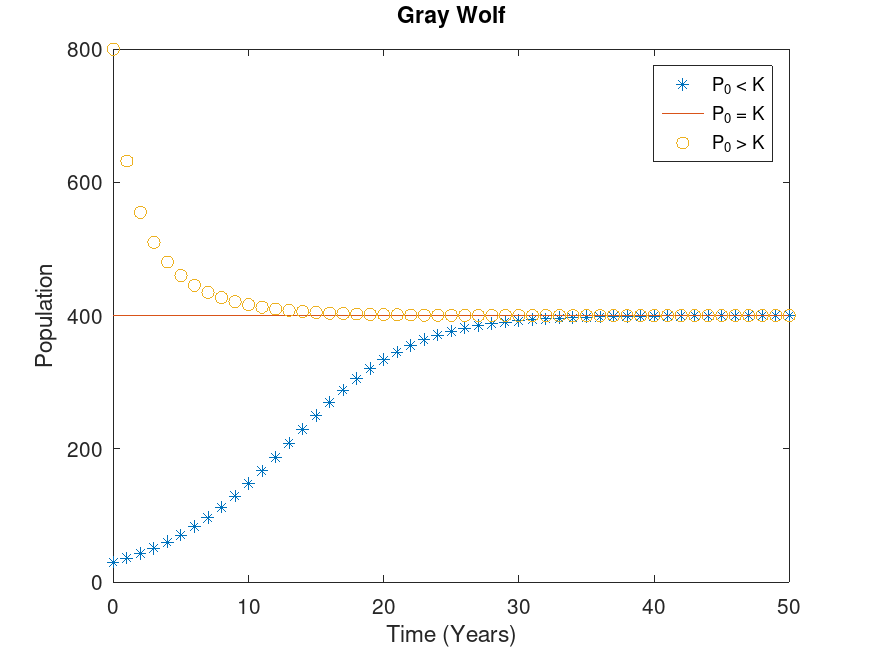
\includegraphics[width=.75\textwidth]{Images/GrayWolf.png}
  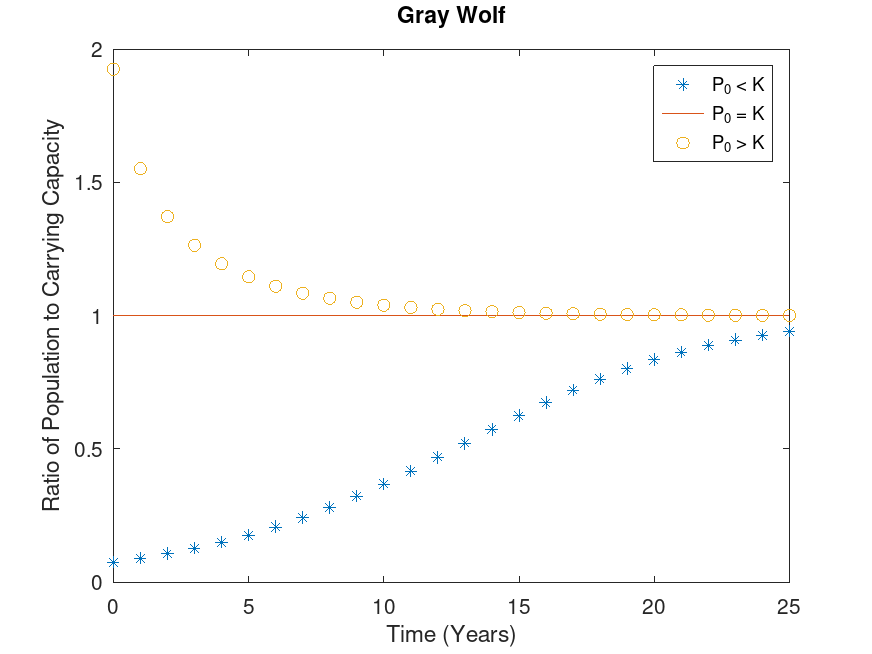
\includegraphics[width=.75\textwidth]{Images/GrayWolfCC.png}
\end{center}

\subsection{Moose}

\begin{center}
  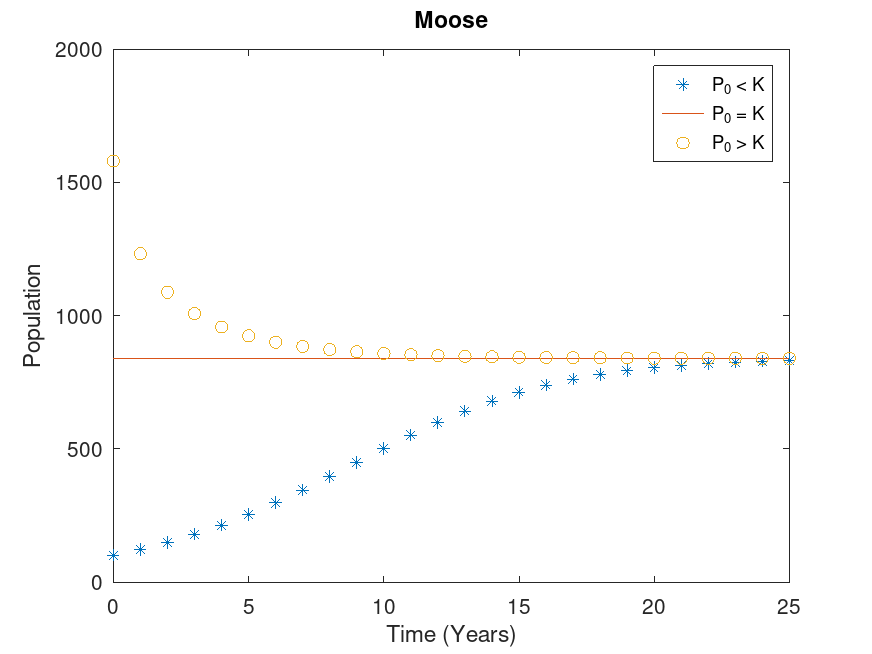
\includegraphics[width=.75\textwidth]{Images/Moose.png}
  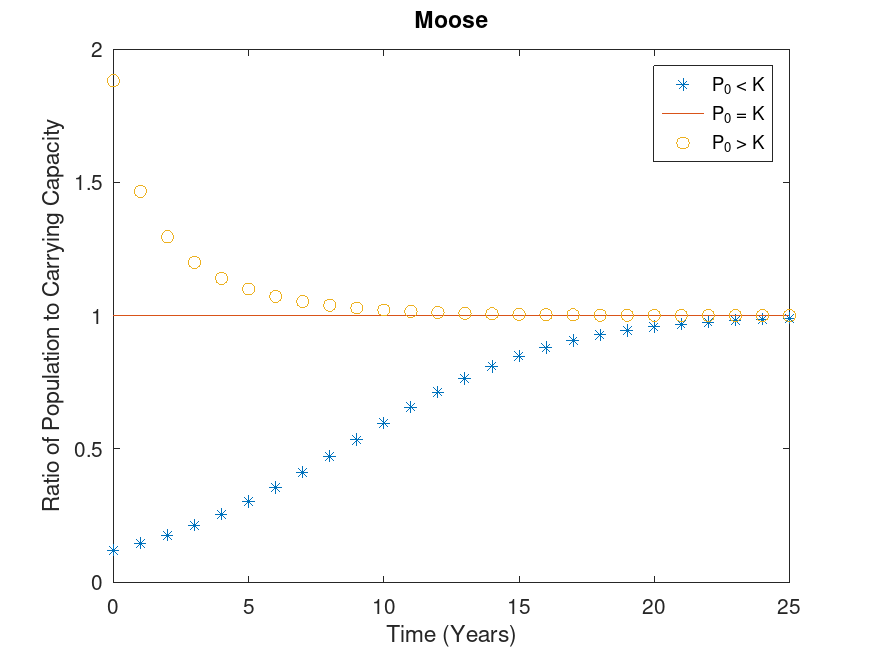
\includegraphics[width=.75\textwidth]{Images/MooseCC.png}
\end{center}

\subsection{Woodland Caribou}

\begin{center}
  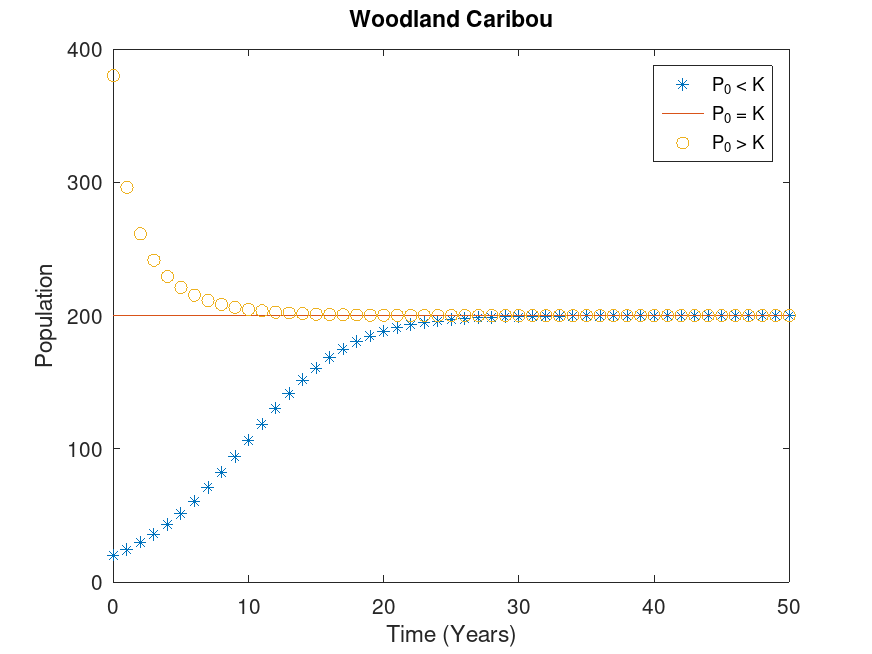
\includegraphics[width=.75\textwidth]{Images/Caribou.png}
  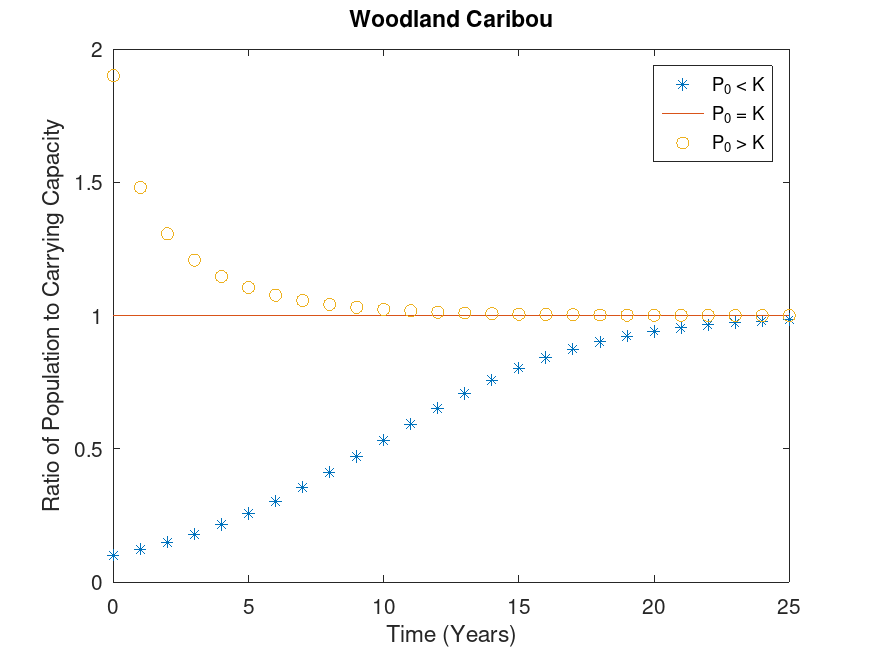
\includegraphics[width=.75\textwidth]{Images/CaribouCC.png}
\end{center}

\subsection{Elephant}

\begin{center}
  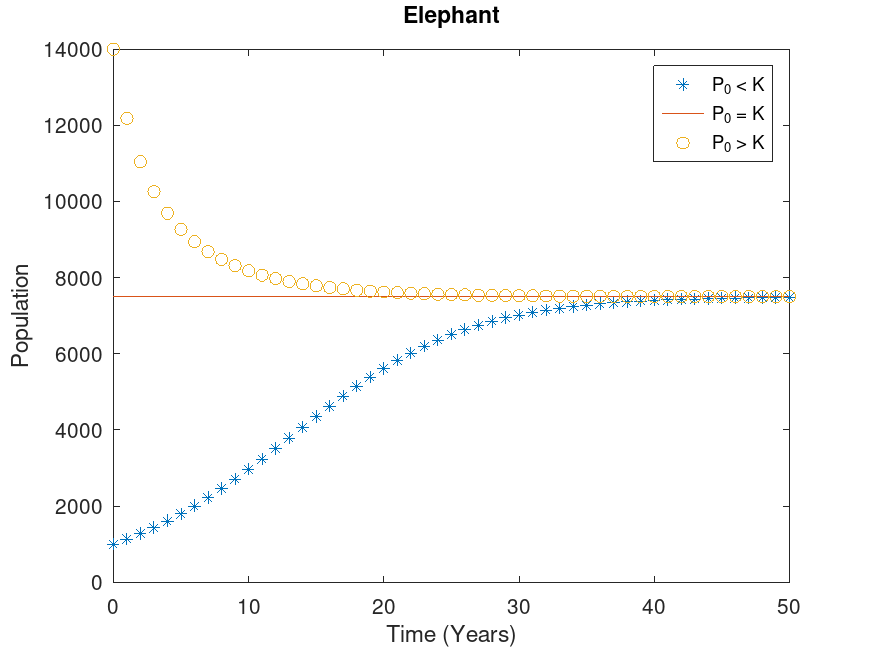
\includegraphics[width=.75\textwidth]{Images/Elephant.png}
  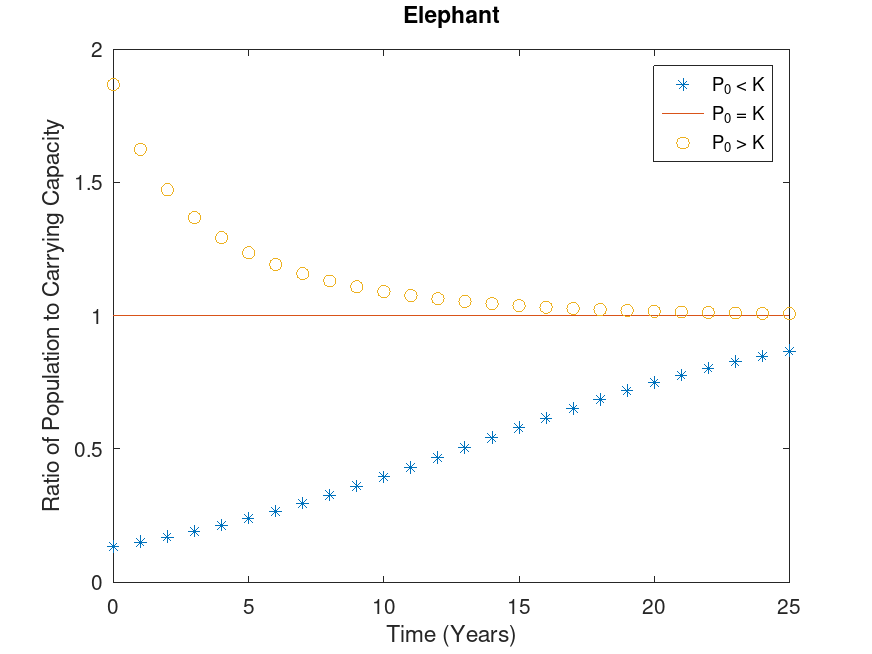
\includegraphics[width=.75\textwidth]{Images/ElephantCC.png}
\end{center}

\end{document}

